%Introduction
\newcommand{\gf}{\textsc{Geant4}\xspace}
\newpage

In this chapter I present a brief introduction of the
LHC physics and the physics behind the off-shell methods
for constraining Higgs decay width.

\section{Physics at LHC}
\begin{itemize}
    \item LHC
    \item CMS (trigger, PF, anti-Kt)
\end{itemize}

After the discovery of Standard Model (SM) Higgs boson in 2012, the Large Hadron Collider (LHC)
went through a series of upgrades during Long Shutdown 1 (2013-2015) and finally restarted with center-of-mass energy reaching
\SI{13}{\tera\electronvolt}. Though the last particle promised by the SM has been discovered,
no SuperSymmetry (SUSY) particle was spotted at all.

The LHC has been operating at the same energy for the past 3 years (2016-2018) and each year
the delivered luminosity as been ramping up.\cite{xampl} In this analysis, we will be using
simulation that corresponds to Run period 2018, which in turn corresponds to a 
\SI{59.74}{\per\femto\barn} luminosity for the Compact Muon Solenoid (CMS) detector.\cite{xampl}


\section{The CMS Detector}
The CMS is one of the two general purpose detectors built around LHC (the other one is ATLAS). It
is `compact' only when comparing to the ATLAS detector and is in fact heavier than the latter.
Though we are not using the data accumulated by the CMS detector, the simulated events are
reconstructed based on the material and electronics responses of the real detector using the
\gf{} package.\cite{geant4}

The defining feature of the CMS detector is the solenoid (as in its name) around the beam line.
This superconducting solenoid produces a \SI{4}{\tesla} magnetic field and is 
\SI{12.5}{\meter} long free bore.\cite{validation of cms} This feature allows the track of
any charged particle (given the momentum is not ridiculously high) to be bent when penetrating
the detector layers and leave behind a track which provides information regarding the particle's 
electric charge.

\begin{figure}[htb]
\begin{center}
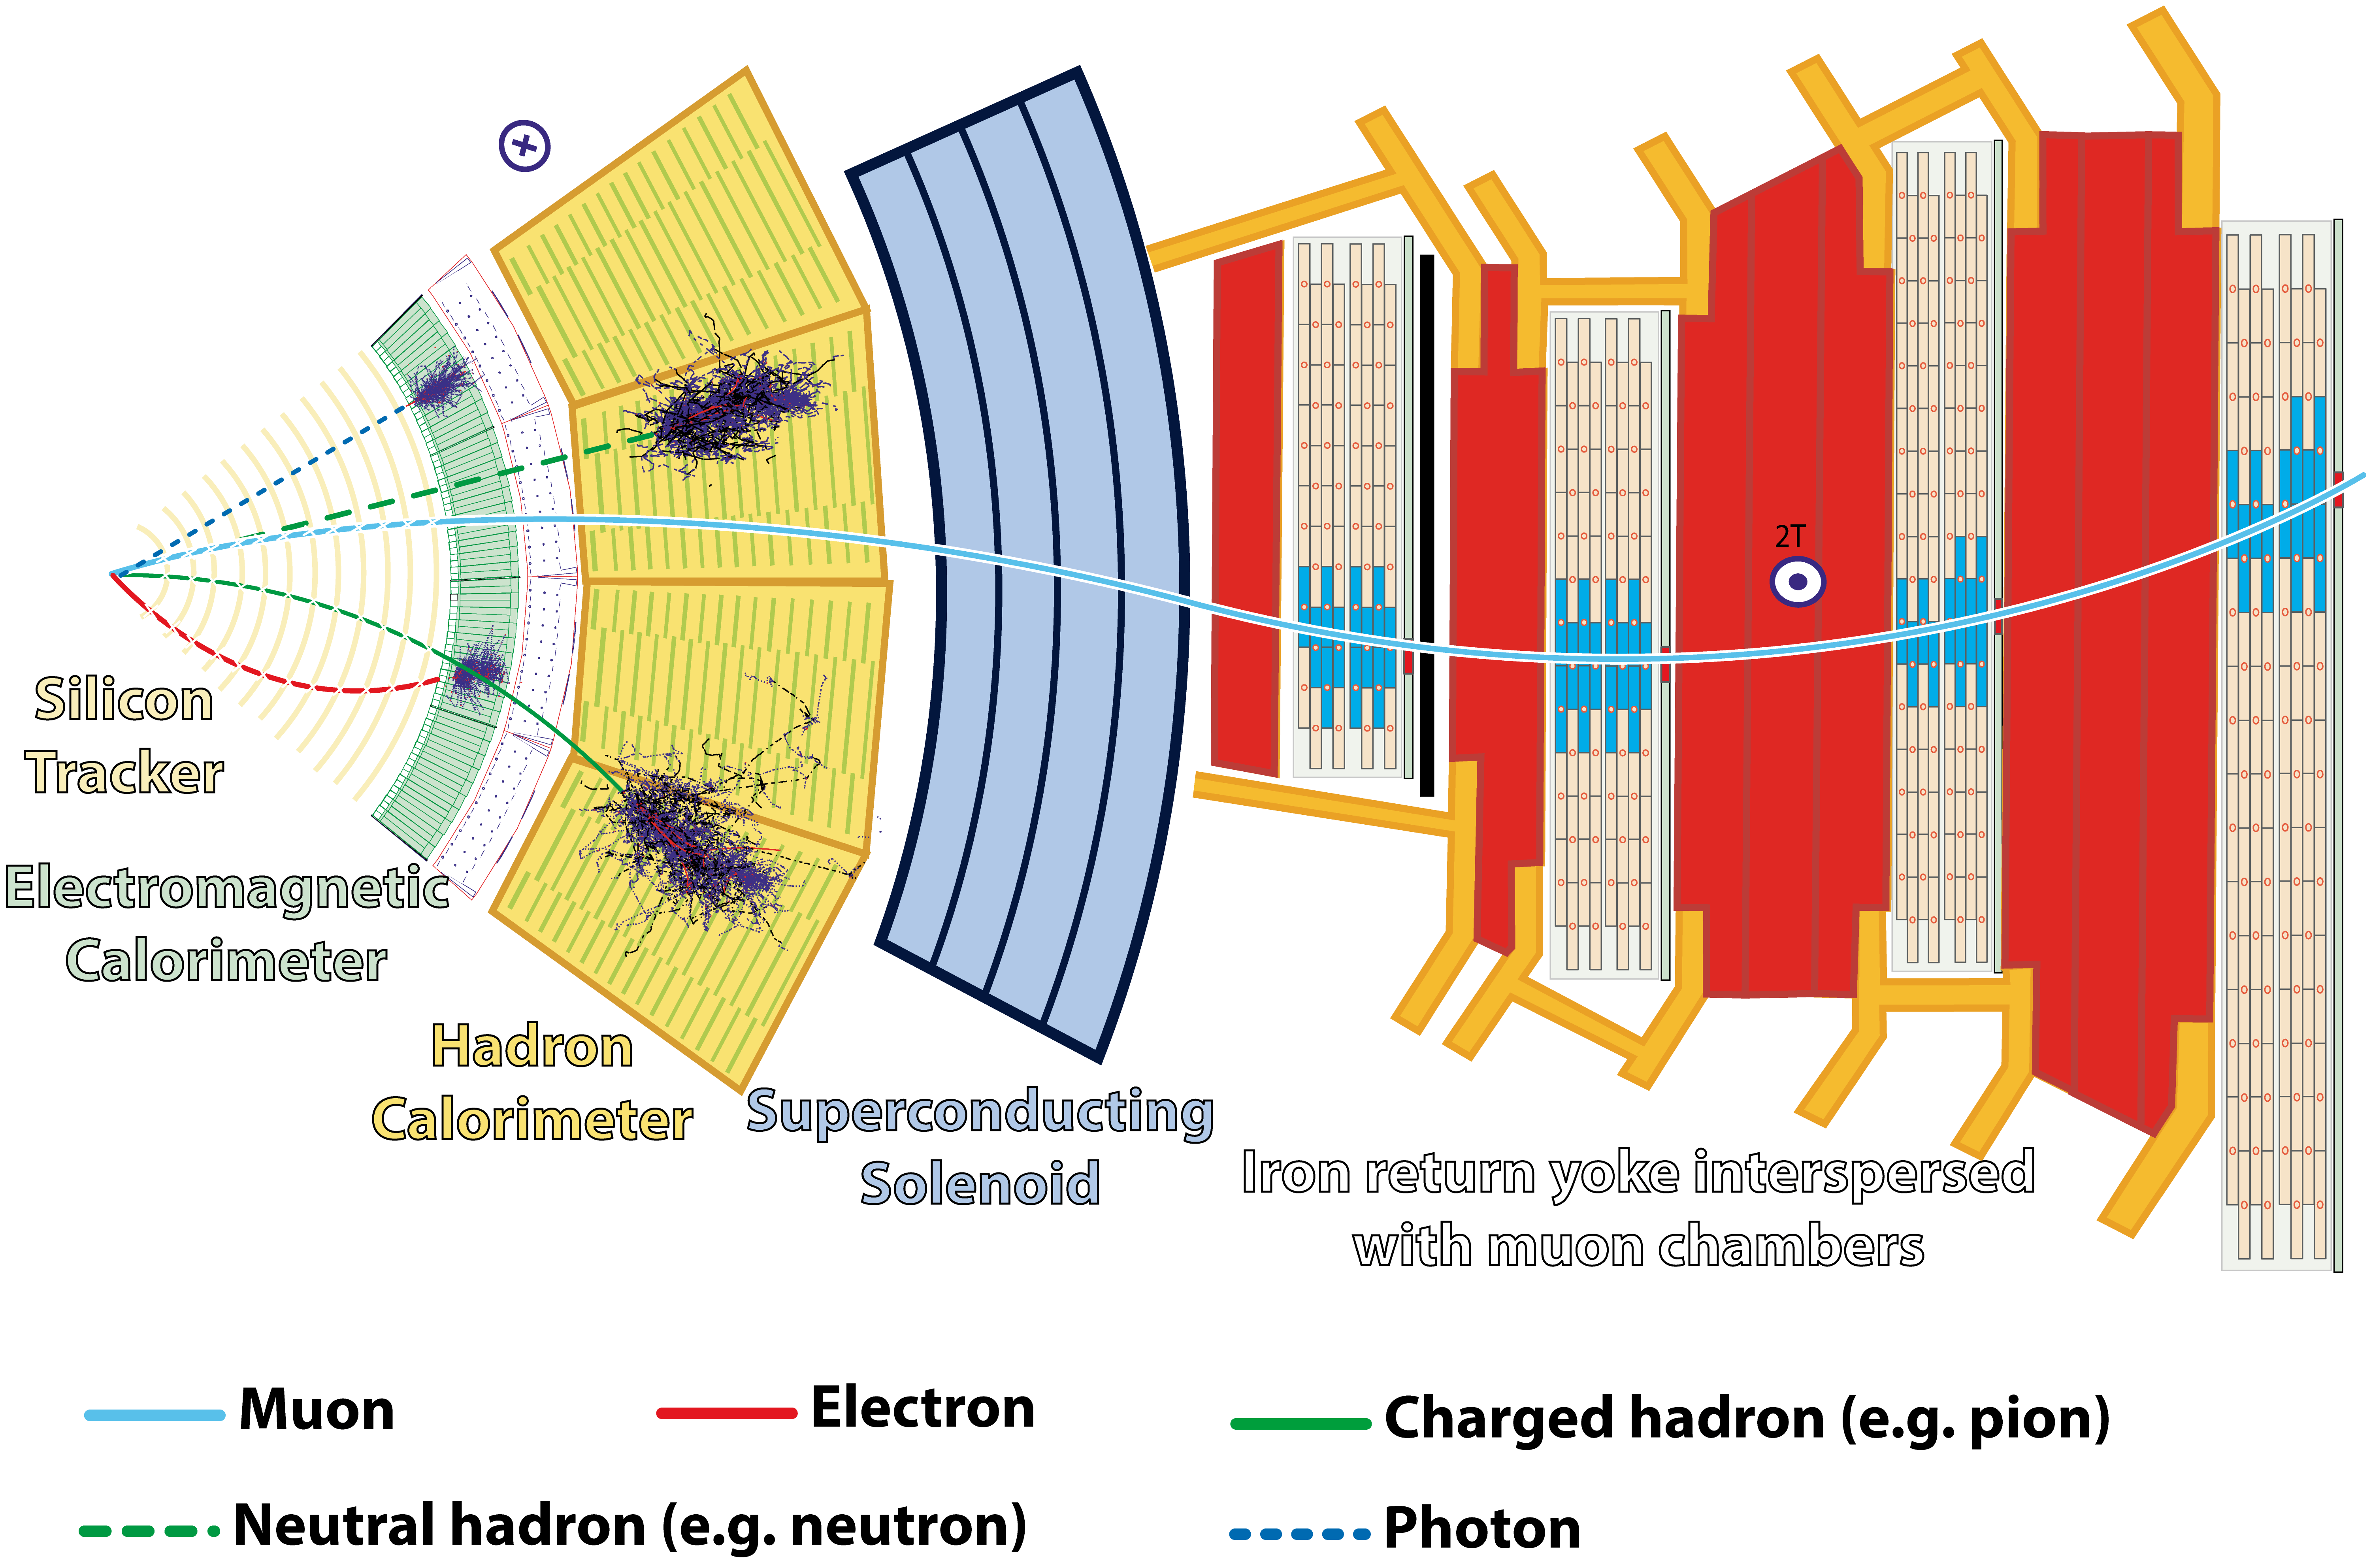
\includegraphics[width=.70\linewidth]{fig/CMS_Slice.png}
\end{center}
\caption{A section slice of the CMS detector where we can see how 
particles with different physical properties interact differently with the detector.}
\label{fig:CMS_Slice}
\end{figure}

One important kind `final-state' particles used in this thesis this charged lepton, 
which includes electrons and muons (half-life of tauon is too short);
`final-state' here means they are the end products of decay chain and interact with detector
components directly. If we concentrate on the red and blue lines in \ref{fig:CMS_Slice}, we
can see that for the electrons (blue), they leave a few hits (4) that resemble a curved
track within the Silicon Tracker layer and are stopped at the Electromagnetic Calorimeter
(ECAL). 

For the muons, they largely go through all the interior layers unhinged due to their
high mass; pay close attention to the `S'-shaped curve, this is due to the opposite magnetic
field outside of the superconducting solenoid. Information regarding muons are largely and 
most reliably extracted from the muon chambers withing the iron return yoke. Notice how the
muon chambers occupy more than half of the detector by size, such design allows the CMS 
detector to exceeds in muon measurements and is the primary reason for the overall design.


\section{The physics of off-shell methods}
[1]Caola F, Melnikov K. Constraining the Higgs boson width with ZZ production at the LHC. Phys Rev D 2013;88:054024. https://doi.org/10.1103/PhysRevD.88.054024.

The importance of a Beyond Standard Model (BSM) physics is self-evident, though the SM is one
of the most precise theory in physics we ever had, the model requires many `inputs' from experiment
for parametrization, and, it cannot account for phenomena such as neutrino oscillation with its
original form. While the direct searches in the past few years have all yield null results,
many in-direct probing have been going as well.
\newpage\phantom{blabla}
\newpage\phantom{blabla}


\section{Background and signal simulation}
[1]Agostinelli S, Allison J, Amako K, Apostolakis J, Araujo H, Arce P, et al. Geant4—a simulation toolkit. Nuclear Instruments and Methods in Physics Research Section A: Accelerators, Spectrometers, Detectors and Associated Equipment 2003;506:250–303. https://doi.org/10.1016/S0168-9002(03)01368-8.

[2]Gritsan AV, Roskes J, Sarica U, Schulze M, Xiao M, Zhou Y. New features in the JHU generator framework. ArXiv:200209888 [Hep-Ex, Physics:Hep-Ph] 2020.

[3]The NNPDF Collaboration, Ball RD, Bertone V, Carrazza S, Deans CS, Del Debbio L, et al. Parton distributions for the LHC Run II. J High Energ Phys 2015;2015:40. https://doi.org/10.1007/JHEP04(2015)040.

[4]Melia T, Nason P, Röntsch R, Zanderighi G. W+W-, WZ and ZZ production in the POWHEG BOX. J High Energ Phys 2011;2011:78. https://doi.org/10.1007/JHEP11(2011)078.

\newpage\phantom{blabla}
\newpage\phantom{blabla}


\section{The CMS detector and event reconstruction}
[1]CMS Collaboration. Performance of CMS muon reconstruction in pp collision events at sqrt(s) = 7 TeV. J Inst 2012;7:P10002–P10002. https://doi.org/10.1088/1748-0221/7/10/P10002.

[2]CMS Collaboration. Performance of electron reconstruction and selection with the CMS detector in proton-proton collisions at sqrt(s) = 8 TeV. J Inst 2015;10:P06005–P06005. https://doi.org/10.1088/1748-0221/10/06/P06005.

[3]Cacciari M, Salam GP, Soyez G. FastJet user manual. Eur Phys J C 2012;72:1896. https://doi.org/10.1140/epjc/s10052-012-1896-2.

[4][0802.1189] The anti-k\_t jet clustering algorithm n.d. https://arxiv.org/abs/0802.1189 (accessed May 25, 2020).


\newpage\phantom{blabla}
\newpage\phantom{blabla}
